\cotefile{156-4}
\scanpage{66}\mspage{65}
Ceci résulte du \deleted{\uline{C}4 et} cor. 1 et du

\uline{Lemme} Pour que $F$ soit de t. f.\inserted{(resp. fini)} il f et s que a) les $F_i$ le soient et b) Tous les $F_i$ sauf un nb fini sont $\varnothing$.

Notations $\pi_0(F)$ (NB Si $F\leq G$ on a $\pi_0(F)\longrightarrow\pi_0(G)$\deleted{\unsure{)|?}}, et transitivité) $\pi_0(M)$, $\pi_0^{\substack{\deleted{\unsure{\mathrm{cat}|\mathrm{act}}}\\!}}(\mathcal F)$. (\unsure{Attention}, le $\pi_0^{\unsure{d|!}}(\mathcal F)$ n'est pas le $\pi_0(F,\leq)$, mais le $\pi_0$ ``en tenant compte du Sup''. Si
% The two notes stand below the tuple and are linked to its C and third relation.
% The third relation is ONE retraced group; the alternatives include its uncertain cancellation state.
\figure{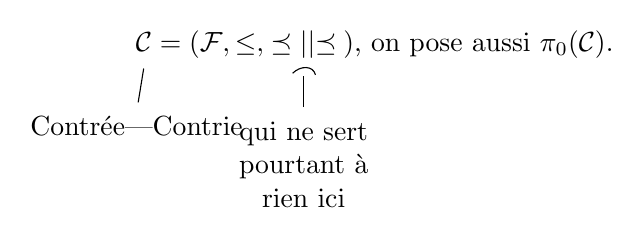
\begin{tikzpicture}[every node/.style={inner sep=1pt}]
  \node[anchor=base west] (prefix) at (0,0) {$\mathcal C=(\mathcal F,\leq,$};
  \node[anchor=base west] (relation) at (prefix.base east) {$\unsure{\preceq|\leqslant|\deleted{\preceq}}$};
  \node[anchor=base west] (rest) at (relation.base east) {$)$, on pose aussi $\pi_0(\mathcal C)$.};
  \draw[thin] (0.14,-0.22) -- (0.07,-0.65);
  \node[anchor=north] at (0.05,-0.79) {\unsure{Contrée|Contrie}};
  \draw[thin] (relation.south) ++(0,-0.58) -- ++(0,0.40);
  \draw[thin] (relation.south) ++(-0.14,-0.15)
    .. controls +(0.10,0.10) and +(-0.03,0.12) .. ++(0.29,-0.02);
  \path (relation.south) ++(0,-0.73)
    node[anchor=north,align=center] {qui ne sert\\\deleted{\unsure{pourtant}} \unsure{à}\\rien ici};
\end{tikzpicture}}

Axiome renforcé

\uuline{C4 bis} Pour tout $(F_i)_i\in\prod\mathcal F_i$, $\deleted{\unsure{\exists F|\exists\mathcal F}}$ $\exists F\in\mathcal F$ telle que $F\mid M_i=\deleted{\unsure{\mathcal F}}F_i$ pour $i\vdash I$,

\uline{\unsure{Contrée|Contrie} résiduelle} \uline{Support} \uline{et} \uline{cosupport}

Soit $\deleted{\unsure{(F_i)\in\mathcal F|(H_i)\in\mathcal F}}$ $\Phi\subset\mathcal F$ un ens. de figures\inserted{$H_i$}. \deleted{On posera} Soit $F$ une figure. Pour \deleted{Cosupp. $\Phi$} que $F$ soit \unsure{disjointe|disjoint} de tous les $H_i$, il f et s. que ce soit le cas pour toutes les strates de $F$ (à cause de C3). \deleted{Posons} Posons
